% Spectroscopic methods span a wide range of regimes and objectives, including optical spectroscopy \cite{schawlow_infrared_1958}, nuclear magnetic (NMR) \cite{PhysRev.70.460,PhysRev.69.37}, electron spin resonance (ESR) and more. Among the most notable advances, \textit{Stimulated Emission Depletion} (STED) microscopy, introduced by Hell, surpasses the diffraction limit of light microscopy by selectively depleting fluorescence around a targeted nanoscale region, achieving resolutions on the order of tens of nanometers \cite{hell_breaking_1994,HELL199419}.  

% Parallel to these advancements, continuous efforts aim to overcome intrinsic spectral broadening mechanisms such as Doppler, Fourier (transit-time), and power broadening~\cite{PhysRevLett.104.053001,finkelstein_power_2019}. However, even in the absence of technical noise, the ultimate spectral resolution of a coherently driven two-level system is fundamentally limited by decoherence. According to the Bloch equations, the homogeneous linewidth scales inversely with the coherence time $T_2$, establishing the so-called $T_2$ limit~\cite{Zienau_1975,PhysRev.70.460}. While various schemes seek to mitigate this constraint through dynamical decoupling or engineered dissipation~\cite{PhysRevLett.122.060503,retzker_2,Cao_2025}, the connection between decoherence and spectral resolution is generally regarded as fundamental, as the same stochastic frequency fluctuations that govern dephasing also determine the resolvability of energy-level transitions.

% Experimentally, this limit is probed by weak-drive spectroscopy, in which a continuous tone is swept across the qubit transition while monitoring the excited-state population\cite{PhysRevLett.107.240501,PhysRevX.9.041041,spec123}. In this regime, the drive amplitude must remain sufficiently small to avoid power broadening, allowing the measured linewidth to approach the intrinsic decoherence-limited value.Increasing the drive strength enhances signal visibility but leads to transition saturation and a corresponding linewidth that grows approximately linearly with the drive amplitude. Conversely, excessively weak driving results in poor signal-to-noise ratio and limits spectral resolvability. As a result, conventional spectroscopy operates within a narrow range of drive amplitudes that balances signal strength against power-induced broadening. 

\begin{figure}
    \centering
    
\includegraphics[width=1\linewidth]{figures/lorentzian_time_and_frequency.png}
    \caption{
    Time and frequency-domain representation of the root-Lorentzian and echo-root-Lorentzian drive pulses.
    (a) Time-domain profiles of a Lorentzian $L_{1/2}$, and echo-Lorentzian $L^{\mathrm{echo}}_{1/2}$ pulse with a $\pi$ phase jump at $t=0$. Red dotted lines indicate the temporal cutoff applied to the pulse envelope. Insets show zoomed-in views of the pulse near the cutoff and phase-jump regions.
    (b) Corresponding amplitude spectra $|\Omega(f)|$. The echo-root-Lorentzian pulse exhibits a suppression of spectral weight around zero frequency due to destructive interference induced by the phase inversion, resulting in a spectral null at resonance. The $T_2$-limited linewidth is indicated by the green dotted line.}
    \label{fig:fig1}
\end{figure}


Accurate frequency characterization of a quantum two-level system (qubit) is essential for calibrating high-fidelity control in fault-tolerant quantum processors. In many physical implementations, such as superconducting circuits and semiconductor quantum dots, the qubit is realized within an inherently multilevel structure with discrete energy levels, allowing two levels to be selected to form an effective computational subspace that mimics atomic systems via their quantized energy spectrum~\cite{PhysRevA.69.062320,PhysRevA.76.042319}. Spectroscopic identification of the transition frequency is therefore routinely performed by applying resonant control fields and monitoring the resulting population dynamics~\cite{PhysRevLett.107.240501,PhysRevX.9.041041,spec123}.
Spectroscopic resolution in coherently driven two-level systems is fundamentally constrained by decoherence. In the absence of technical noise, stochastic phase fluctuations induce homogeneous broadening of the transition frequency, leading to a minimum resolvable linewidth that scales inversely with the coherence time $T_2$, as described by the Bloch equations~\cite{PhysRev.70.460,Zienau_1975}. This establishes the so-called $T_2$ limit, which is generally regarded as a fundamental bound on the spectral distinguishability of energy-level transitions.




In practice, however, driven spectroscopy introduces an additional trade-off between signal robustness and spectral resolution. When finite-amplitude control pulses are applied, the system dynamics deviate from the idealized two-level response due to coherent Rabi oscillations and coupling to noncomputational levels. Increasing the drive amplitude improves signal contrast and robustness against state-preparation and measurement errors, but simultaneously induces power broadening, resulting in a linewidth that scales with the instantaneous Rabi frequency. Consequently, conventional spectroscopic techniques must operate at low drive amplitudes in order to maintain resolution approaching the decoherence-limited linewidth set by $T_2$, rendering precision and robustness fundamentally incompatible.






Ramsey interferometry provides a standard alternative to direct spectroscopy and, in principle, enables frequency estimation at the $T_2$ limit. Achieving such resolution, however, requires long interrogation times and sufficiently dense temporal sampling to resolve the resulting interference fringes. Moreover, Ramsey measurements are susceptible to systematic biases: asymmetries in the exponential decay envelope—arising, for example, from pulse miscalibration—can shift the apparent resonance peak in the frequency domain. Additional effects such as phase fluctuations or unintended AC Stark shifts during the control pulses introduce further distortions, ultimately biasing the extracted transition frequency.

Continuous efforts aim to mitigate this trade-off through dynamical decoupling or engineered dissipation~\cite{PhysRevLett.122.060503,retzker_2,Cao_2025}. However, these approaches typically require extended interrogation times or additional control resources, and do not overcome the intrinsic connection between decoherence and spectral resolution, as the same stochastic frequency fluctuations that govern dephasing also determine the resolvability of the transition frequency. Here, we show that this limitation can be bypassed in the driven regime by employing adiabatically engineered Lorentzian-derived drive pulses with a $\pi$-phase inversion at their peak. This echo-like structure suppresses on-resonant Rabi oscillations while preserving the steady-state spectral response, enabling $T_2$-limited frequency characterization at drive amplitudes exceeding those used in conventional spectroscopy by more than three orders of magnitude.




% In the context of superconducting circuits, circuit quantum electrodynamics (cQED) employs nonlinear harmonic oscillators—most prominently the transmon—to resolve transitions between the ground and excited states of weakly anharmonic systems. This technique, known as qubit spectroscopy, serves as a cornerstone for the calibration and characterization of superconducting quantum processors 

% Ramsey interferometry is a standard alternative to direct spectroscopy. In a typical Ramsey sequence, two $\pi/2$ pulses are separated by a free-evolution interval $\tau$, resulting in interference fringes in the excited-state population that oscillate at the detuning frequency. In practice, however, achieving $T_2$-limited spectral resolution requires both long interrogation times and sufficiently high temporal sampling to resolve the resulting oscillations. Moreover, the accuracy of Ramsey measurements is susceptible to systematic biases: asymmetries in the exponential decay envelope—arising, for example, from pulse miscalibration—can shift the perceived resonance peak in the frequency domain. Additional effects such as phase fluctuations or unintended AC Stark shifts during the control pulses introduce further distortions, ultimately biasing the extracted frequency estimate.\cite{PhysRevA.98.053424,PhysRev.78.695,wang_coherent_2019}.

\begin{figure}
    \centering
    
\includegraphics[width=1\linewidth]{figures/2d_spectroscopy_comparison.png}
    \caption{
Two-dimensional spectroscopy of the excited-state population as a function of detuning $\Delta$ and drive amplitude $\Omega_0$ for three pulse types: (a) square, (c) root-Lorentzian, and (e) echo- root-Lorentzian pulses. Panels (b), (d), and (f) show detuning line cuts at selected amplitudes $\Omega_0/2\pi$, as indicated in the corespondent colored ticks on the left column plots. Vertical dashed lines denote the $T_2$ limit line width. The square pulse exhibits strong power broadening already at small amplitudes ($\Omega_0/2\pi\sim0.05$~MHz), whereas the root-Lorentzian and echo-type pulse (30~$\mu$s) maintain narrow, $T_2$-limited linewidths. The echo-type pulse further suppresses coherent vertical oscillations, enabling smooth high-resolution spectroscopy all over the the amplitude range, but with an expense of SNR.   
    }
    \label{fig:fig2}
\end{figure}

\begin{figure}
    \centering
    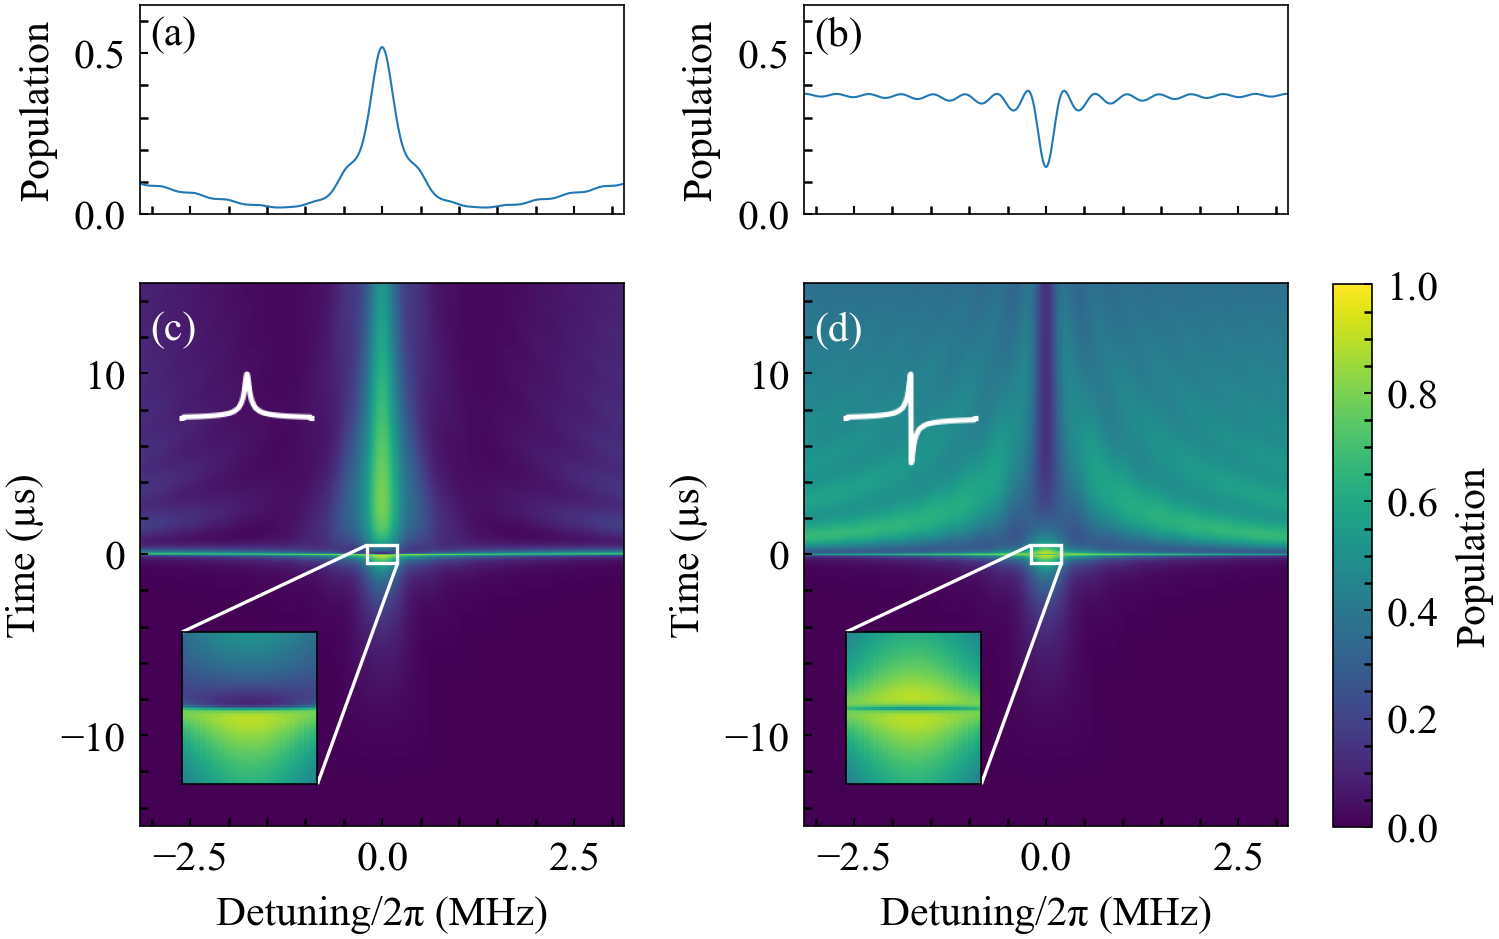
\includegraphics[width=1\linewidth]{figures/2d_spectroscopy_simulation.png}
    \caption{  Numerical simulation of qubit spectroscopy under a root-Lorentzian drive and its echo variant. (a) Final excited-state population as a function of detuning $\Delta/2\pi$ for a standard root-Lorentzian pulse. (b) Same for the echo-root-Lorentzian pulse $L^{(1/2)}_{\mathrm{echo}}$. (c),(d) Full time evolution of the excited-state population versus detuning for the corresponding drives. The pulse duration is $30~\mu\mathrm{s}$ with a cutoff of $5\times10^{-4}$. While the standard pulse yields a resonant peak at zero detuning, the echo sequence produces an inversion of the central response, leading to a pronounced dip. This behavior reflects cancellation of coherent oscillations at $\Delta=0$, as highlighted in the insets. 
    }

    \label{fig:fig3}
\end{figure}


Precise determination of the qubit transition frequency is crucial for implementing high-fidelity quantum gates. The drive frequency must coincide with the qubit resonance, as detuning directly reduces gate fidelity. A rigorous metric for quantifying such calibration errors is the diamond norm, which captures deviations in the implemented quantum operation from the ideal one. Minimizing these detuning-induced errors is essential to meet the fault-tolerance thresholds required for scalable quantum computation. \cite{diamond}

Here, we propose a spectroscopic method for probing the qubit transition frequency using arbitrarily shaped drive pulses, specifically an echo-root-Lorentzian pulse. In previous works by Vitanov \cite{boradjiev_power_2013}, it was shown that Lorentzian pulses exhibit power-narrowing, complementary to the conventional power broadening observed for constant drives, originating from the adiabatic properties of these pulses. In this work, we extend the analysis of Vitanov to longer pulse durations approaching the $T_1$ timescale, thereby entering a regime beyond the Fourier limit. The echo property arises from a $\pi$-phase jump applied at the peak amplitude of the pulse, which  effectively cancels its net area, while preserving the adiabatic properties of the drive. This phase inversion reverses the coherent phase accumulation at resonance, suppressing on-resonant excitation while maintaining an off-resonant spectral response across the frequency domain, and thus making resonance distinguishable.

We define the root-echo-Lorentzian $L_{\text{echo}}^{(1/2)} $ drive envelope base on ordered Lorentzian $L^{(1/2)}$ as
\begin{align}
L^{(n)}(t)
&= \frac{1}{\left[1+\left(\frac{t}{\tau}\right)^2\right]^n},
\\
L^{(1/2)}_{\mathrm{echo}}(t)
&:= L^{(1/2)}(t)\,\mathrm{sgn}(t).
\label{eq:Ln}
\end{align}
where $\tau$ sets the characteristic pulse duration and $n$ controls the temporal sharpness.

Under the adiabatic condition for the plain Lorentzian pulse, the characteristic spectral width obeys the scaling
\begin{equation}
\Delta_{1/2}\tau
\propto
(\Omega_0 \tau)^{-\frac{1}{2n-1}},
\label{eq:lorentzian_adiabatic}
\end{equation}
where $\Delta_{1/2}$ denotes the typical linewidth and $\Omega_0$ is the peak Rabi frequency. This relation indicates that increasing the drive amplitude suppresses the detuning at which adiabaticity breaks down, resulting in a narrowing of the effective spectral response. In contrast, the square pulse is fully governed by conventional power broadening, for which the linewidth increases approximately linearly with the drive amplitude $\Delta_{1/2}\propto\Omega_0$. This contrast highlights that the spectroscopic response is not determined solely by the drive strength, but depends sensitively on the temporal envelope of the control pulse, motivating the use of tailored pulse shapes \cite{VITANOV2001117,HALFMANN2003353,PhysRevA.70.053407,PhysRevA.57.79,PhysRev.40.502}.

Spectroscopy results obtained using the echo–root-Lorentzian pulse, together with standard square and root-Lorentzian pulses for comparison, are shown in Fig. \ref{fig:fig2}. For the measured coherence time $T_2 \approx 14~\mu\mathrm{s}$,
the corresponding coherence-limited linewidth is
$\Delta_{1/2}/2\pi \approx 20~\mathrm{kHz}$. This limit is indicated by a dotted white line in the two-dimensional amplitude--detuning sweep and by gray dashed lines
in one-dimensional spectroscopy slices extracted at constant drive amplitude.

Square pulses exhibit pronounced power broadening even at low drive
amplitudes compared to Lorentzian-type pulses, with substantial linewidth
expansion observed over three orders of magnitude in amplitude.  In contrast, the root-Lorentzian pulse displays the characteristic power-narrowing behavior, enabling resolution approaching the $T_2$-limited linewidth. However, for pulse durations comparable to the qubit lifetime $T_1$, coherent oscillations arise for both square and root-Lorentzian pulses,
resulting in amplitude-dependent linewidth variations that hinder precise
spectral extraction.

Introducing a $\pi$ phase inversion at the peak of the root-Lorentzian envelope partitions the drive into two sequential segments of opposite phase, such that the corresponding forward and backward evolutions cancel exactly at zero detuning. This echo-like structure suppresses resonant Rabi oscillations while preserving the off-resonant spectral response, producing a sharp depletion feature centered at the qubit transition frequency. \ref{fig:fig1}) In the frequency domain, this manifests as a splitting of the spectral response accompanied by a null at resonance, rendering the measured linewidth largely insensitive to drive amplitude. Formally, this mechanism is equivalent to a Loschmidt-echo–type evolution, in which reversibility is achieved only on resonance, while detuning or decoherence breaks the cancellation and restores excitation. Combined with the adiabatic following ensured by the Lorentzian envelope, this interference effect suppresses both power broadening and coherent Rabi oscillations, enabling spectroscopy approaching the $T_2$-limited linewidth over a broad range of drive strengths and with pulse durations substantially shorter than those required by standard spectroscopy or Ramsey interferometry.

Fig. \ref{fig:fig3} shows a numerical simulation of the qubit state evolution during the spectroscopy echo-root-Lorentzian sequence. At resonance, where the adiabatic condition breaks down, coherent Rabi oscillations are induced by the drive. However, due to the $\pi$ phase inversion at the pulse maximum, the subsequent segment of the drive reverses the accumulated evolution, resulting in a symmetric cancellation that returns the qubit close to the ground state, limited by relaxation ($T_1 = 30~\mu\mathrm{s}$).

For detuned drives, the system remains in the adiabatic regime throughout most of the pulse duration and undergoes excitation only in the vicinity of the pulse peak, where the phase inversion occurs. In this case, the evolution does not cancel and results in a net population transfer followed by relaxation. As a consequence, different detunings produce distinguishable final states, forming the basis of the spectroscopic response.

% Introducing a sign inversion in the root-Lorentzian envelope produces
% an effective $\pi$ phase shift in the drive, leading to a splitting of the
% carrier frequency in the spectral domain. The resulting Fourier spectrum is approximately flat in the vicinity of the qubit transition while exhibiting a null at resonance (see Fig.. This spectral structure implies that, when scanning the drive frequency, the measurement effectively probes a depletion response: excitation is suppressed at resonance and enhanced off-resonantly, producing a spectroscopic “shadow” centered at the transition frequency. In this sense, the qubit response is inferred from the absence of excitation rather than its presence.

\begin{figure}
    \centering
    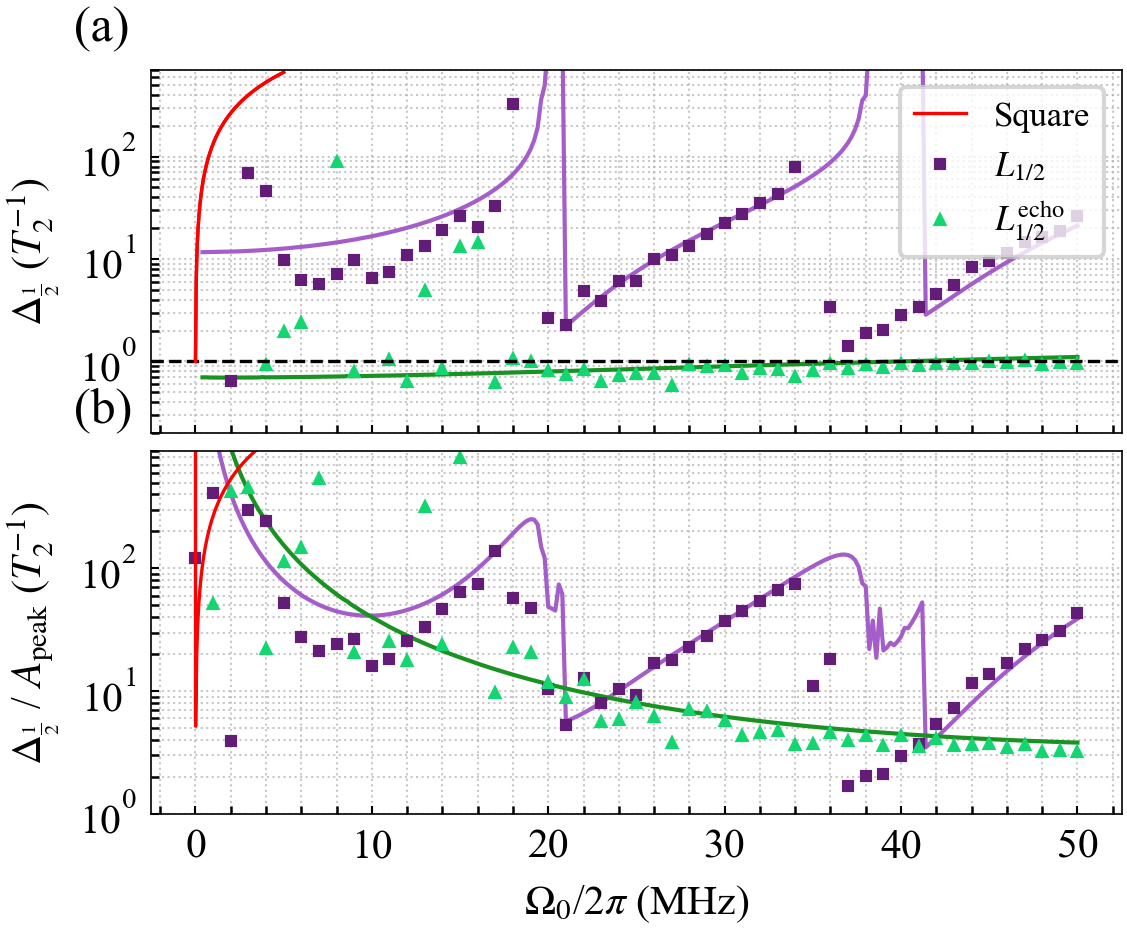
\includegraphics[width=1\linewidth]{figures/fwhm_vs_rabi_prl.png}
    \caption{
    Comparison of spectroscopic linewidth obtained using a constant (square), Lorentzian $L^{(1/2)}$, and echo-Lorentzian $L_{\text{echo}}^{(1/2)} $ drive as a function of peak Rabi frequency $\Omega_0$.
    (a) Measured full width at half maximum (FWHM) $\Delta_{1/2}$ of the qubit spectral response, normalized to the $T_2^{-1}$ limit, together with numerical simulations. Solid lines denote simulation results, while markers represent experimental data. The constant drive (red) exhibits conventional power broadening $\Delta_{1/2}\propto\Omega_0$, whereas the Lorentzian (green) and echo-Lorentzian (purple) pulses display power narrowing due to adiabatic following.
    (b) Linewidth-to-signal ratio $\Delta_{1/2}/A_{\text{peak}}$, highlighting the improved resolution--signal trade-off enabled by the echo-Lorentzian protocol at increasing drive amplitude.
    }

    \label{fig:fig4}
\end{figure}

% This mechanism is conceptually analogous to the principle underlying STED microscopy, in which a doughnut-shaped depletion beam suppresses fluorescence everywhere except at a nanoscale central node where the intensity vanishes. By scanning this engineered intensity null across the sample, fluorescence is confined to a sub-diffraction region, enabling spatial resolution beyond the diffraction limit.

% Moreover, this phase-inverted variant structure closely resembles a Loschmidt-echo–type protocol, which quantifies the reversibility of quantum dynamics under perturbations \cite{Gorin_2006,PhysRevA.30.1610}. The echo signal is defined as
% \begin{equation}
% M(t) = \left| \langle \psi_0 | e^{-i H_2 t} e^{-i H_1 t} | \psi_0 \rangle \right|^2,
% \end{equation}

% where  $H_1$  and $H_2$ denote the forward and backward Hamiltonians, respectively. Perfect time reversal ($H_2 = H_1$) yields $M(t) = 1$, while deviations—arising from detuning or noise—lead to a decay governed by decoherence processes. In our implementation, $H_1$ and $H_2$ correspond to two sequential drive segments of opposite phase, such that full reversibility is achieved only at zero detuning.
  


% Second, the echo property, implemented via a $\pi$ phase inversion at the peak of the pulse, acts as a coherent refocusing mechanism. Whereas a standard Lorentzian pulse ultimately suffers from power broadening with increasing drive strength, the phase jump reverses the accumulated phase at resonance and splits the spectral response. As a result, a destructive interference condition emerges at the carrier frequency: only at zero detuning does the forward and backward evolution cancel exactly, giving rise to a sharp and amplitude-robust null—a spectroscopic dark state. 

% The effectiveness of the echo-type Lorentzian pulse arises from two complementary mechanisms. First, the adiabatic nature of the Lorentzian envelope ensures that over a broad range of drive amplitudes the qubit state follows the instantaneous dressed eigenstate of the driven Hamiltonian. In contrast to square pulses—which introduce abrupt non-adiabatic transitions and induce oscillatory Rabi dynamics—the smooth Lorentzian profile suppresses spectral leakage and mitigates the sidebands typically associated with high-power drives.

In Fig.~\ref{fig:fig4}, we plot the extracted spectroscopic linewidth obtained from Gaussian fits to the measured response. Although the spectral lineshape of a driven two-level system is often expected to follow a Lorentzian profile, the interference-based structure of the present protocol results in a more complex response. In this regime, Gaussian fitting provides a robust and consistent estimate of the linewidth while yielding values comparable to those obtained from Lorentzian fits within our resolution requirements.

We compare the experimentally acquired linewidth extracted from two-dimensional frequency–amplitude sweeps with numerical simulations of an effective two-level system using identical system parameters. The square (red), Lorentzian (green), and echo-Lorentzian (purple) drives are shown, where solid lines denote simulation results and markers represent experimental data. For the square pulse, only simulated results are displayed, as the agreement with experiment was independently validated. We plot both the linewidth $\Delta_{1/2}$ and the linewidth-to-signal ratio $\Delta_{1/2}/A_{\mathrm{peak}}$ to quantify the resolution–signal trade-off.

To suppress residual power broadening at large drive amplitudes the pulse envelope must satisfy requirements on its cutoff behavior. The cutoff effectively introduces a discontinuity in the envelope derivative, effectively behave as a constant pulse, producing a linear broadening that scales with the instantaneous amplitude at the cutoff point, denoted $\Omega_c$. For $T_2$ limited spectroscopy the $T_2$ limit  $T_2^{-1}\leq\Delta_{\frac{1}{2}}$ therefore yields a constraint on the maximum allowable cutoff amplitude $\Omega_c<T_2^{-1}$. In our system Satisfying the above inequality requires a relative cutoff level on the order of $10^{-4}$ to $ 10^{-5}$ depending on pulse duration and peak drive amplitude. Empirically, we find that a cutoff less then $10^{-3}$ is sufficient to eliminate excess broadening and to maintain spectroscopy in the $T_2$ limited regime even under strong driving conditions. See Supplemental material [999].


\begin{figure}
    \centering
    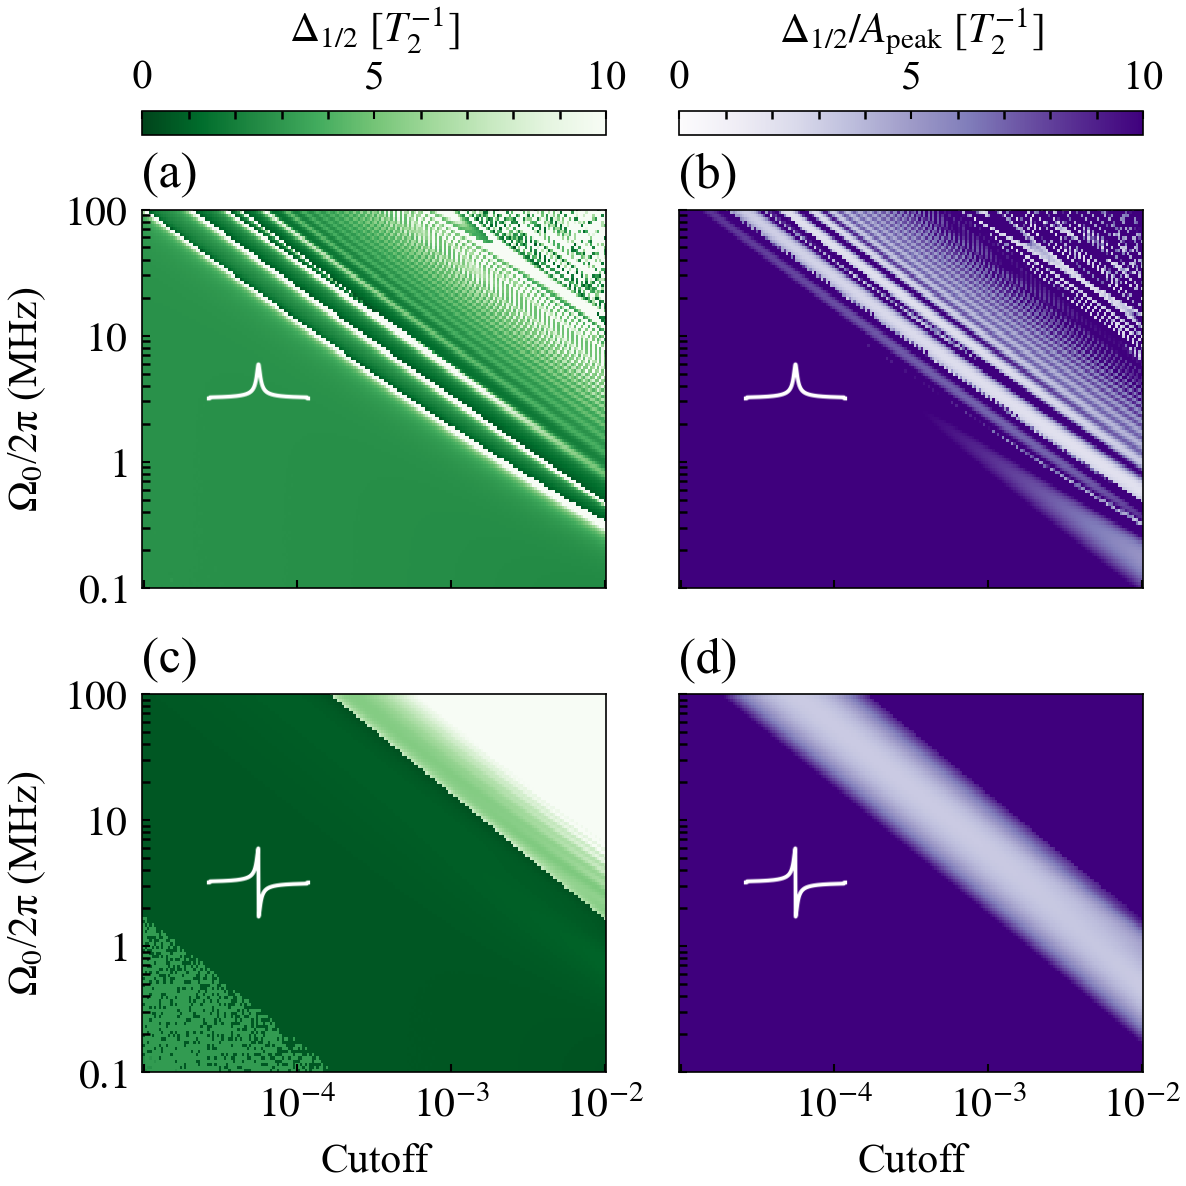
\includegraphics[width=1\linewidth]{figures/spectroscopy_fwhm_snr_vs_amplitude_vs_cutoff_2x2.png}
    \caption{
    Numerical simulation of spectroscopy scans using root-Lorentzian $L^{1/2}$ and echo-root-Lorentzian $L^{(1/2)}_{\text{echo}}$ drives with a pulse duration of $50~\mu\mathrm{s}$.
    (a),(b) Line width $\Delta_{1/2}$ and the linewidth-to-signal ratio $\Delta_{1/2}/A_{\mathrm{peak}}$ obtained using the root-Lorentzian pulse $L^{(1/2)}$ as a function of peak Rabi frequency $\Omega_0$ and temporal cutoff.
    (c),(d) Corresponding results for the echo-root-Lorentzian pulse $L_{\mathrm{echo}}^{(1/2)}$.
    While $L^{(1/2)}$ pulse exhibits extended regions of narrow linewidth, the associated linewidth-to-signal ratio displays strong oscillatory behavior, making it difficult to identify robust operating parameters for high-resolution spectroscopy. In contrast, the echo  variant $L_{\mathrm{echo}}^{(1/2)}$ yields both reduced linewidth and a broad parameter region in which the resolution--signal trade-off remains favorable, enabling stable narrowband spectroscopy.
    }
    \label{fig:fig4}
\end{figure}


% An echo-type sequence applied to the root pulse partially mitigates decoherence effects but remains limited by pronounced amplitude-dependent broadening. Conversely, the Lorentzian echo variant demonstrates an amplitude-independent linewidth spanning over three orders of magnitude in drive strength, evidencing remarkable robustness against amplitude-induced dephasing. This insensitivity arises from the adiabatic evolution and the symmetric frequency-splitting intrinsic to the pulse design. The primary limitation lies in the floating offset and amplitude-dependent baseline, resulting in reduced signal-to-noise ratio compared to conventional square and Lorentzian drives.



At the core of assessing pulse quality and identifying optimal operating regimes lies the spectral response of the driven qubit. We find that the echo pulse yields spectroscopic features with markedly reduced linewidths over a well-defined region of parameter space. In particular, the pulse duration must remain shorter than the qubit lifetime $T_1$, while exceeding approximately $10~\mu s$ in order to suppress Fourier-limited broadening (see Supplemental Material [999]).

This constitutes an additional advantage of the echo protocol. While both constant and simple Lorentzian pulses exhibit coherent Rabi oscillations that persist even for pulse durations comparable to or exceeding $T_1$, the intrinsic $\pi$-phase inversion of the echo pulse suppresses these coherence-induced oscillations. As a result, the spectral response remains smooth and well-behaved, enabling reliable linewidth extraction in regimes where standard and Lorentzian pulses display pronounced oscillatory distortions. (see Supplemental Material [999]).

Second, the use of formally infinite-support pulses necessitates the introduction of a cutoff parameter, as discussed previously. Consequently, the relevant parameter space is effectively three-dimensional: pulse duration, drive amplitude, and cutoff level.

Motivated by the stability observed at fixed pulse duration, we restrict the analysis to constant-length pulses and examine the remaining two parameters. In Fig. 4 we simulate both the root-Lorentzian pulse and its echo-modified counterpart. We extract the full width at half maximum (FWHM) via fitting (as in Fig. 3) and evaluate the normalized metric given by the linewidth divided by the peak signal amplitude. This quantity is strongly correlated with spectral resolution and is directly connected to the inverse Fisher information, i.e., the Cramér–Rao bound.

The results reveal that the root Lorentzian pulse achieves narrow linewidths across a relatively large region of parameter space. However, its performance is not uniform and exhibits oscillatory structure for the chosen pulse duration. In contrast, the echo-root Lorentzian pulse produces even narrower linewidths while maintaining a significantly broader and more uniform high-resolution region. Although the optimal region may appear small at first glance, the logarithmic scale of the parameter axes should be noted. More importantly, the high-resolution region forms a robust and contiguous “island,” indicating strong parameter insensitivity. This robustness makes the echo protocol substantially more stable against parameter variations and therefore highly advantageous for practical spectroscopy.


In conclusion, we have demonstrated that the echo–Lorentzian pulse constitutes a promising and practical approach for high-resolution spectroscopy. By combining adiabatic shaping with an intrinsic echo phase inversion, the protocol significantly enhances robustness against drive-amplitude variations. Remarkably, it broadens the operational amplitude window by approximately three orders of magnitude, while maintaining high spectral resolution even at drive strengths approaching neighboring qubit transitions. These properties make the echo–Lorentzian protocol particularly attractive for precision qubit characterization under realistic experimental constraints.

This opens the route to coherent spectroscopy based on phase-sensitive off-resonant response rather than population transfer.









